
\frame{
\frametitle{¿Qué es un GPU (Graphics Processing Unit)?}
\begin{columns}
\begin{column}{0.79\textwidth}
\begin{itemize}
\item Un GPU es un procesador formado por muchos núcleos más pequeños y especializados.
\item Al trabajar conjuntamente, los núcleos ofrecen un desempeño masivo cuando se puede dividir una tarea de procesamiento y es procesada por muchos núcleos.
\end{itemize}
\end{column}
\begin{column}{0.19\textwidth}
\begin{center}
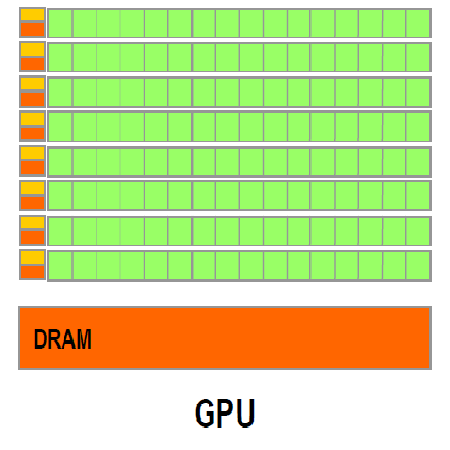
\includegraphics[width=0.9\textwidth]{Figs/GPU}\\
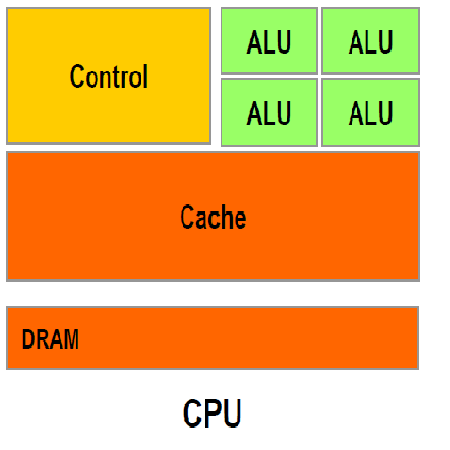
\includegraphics[width=0.9\textwidth]{Figs/CPU}\\
\end{center}
\end{column}
\end{columns}
}




\begin{frame}{Mobile CPUs and SOCs}
\begin{columns}
\begin{column}{0.60\textwidth}  
\begin{itemize}
\item La mayoría de los teléfonos inteligentes tienen procesadores multicore
\item Un CPU aún cuando es rápido, no esta diseñado para manejar de manera eficiente operaciones de punto flotante. 
\item Un CPU no tiene el suficiente poder de cómputo para generar gráficos en 3D complejos en tiempo real. 
%\item Un GPU es una unidad especializada de procesamiento para operaciones de punto flotante en paralelo.
%\item El Samsung S10 Qualcomm Snapdragon 855 SoC (tiene un CPU de 8 núcleos y un GPU dedidado para gráficos (Adreno 640).
\end{itemize}
\end{column}
\begin{column}{0.40\textwidth}  
    \begin{center}
     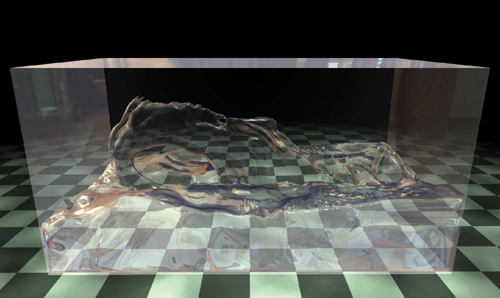
\includegraphics[width=\textwidth]{Figs/Nvidia_Fluido.jpg}\\
          
\includegraphics[width=\textwidth]{Figs/Nvidia_FleX_cereal.jpg}\\
     \end{center}
\end{column}
\end{columns}
\end{frame}


\begin{frame}{SoCs para Teléfonos Inteligentes}
\begin{columns}
\begin{column}{0.60\textwidth}  
\begin{itemize}
\item El término SoC significa system-on-a-chip.
\item Un SoC es un sistema completo contenido en un solo circuito integrado.
\item La combinación de todos sus componentes en una sola unidad de procesamiento permite un ahorro de energía significativo. 
\item Bloques comunes en un SoC:
\begin{itemize}
\item Central Processing Unit (CPU).
\item Graphics Processing Unit (GPU).
\item Image Processing Unit (ISP).
\item Digital Signal Processor (DSP).
\item Neural Processing Unit (NPU).
\item Video encoder/decoder.
\item Modems.
\end{itemize}
%\item La mayoría de los teléfonos inteligentes tienen integrado un GPU
%\item Un GPU es una unidad especializada de procesamiento para operaciones de punto flotante en paralelo.
%\item El Samsung S10 Qualcomm Snapdragon 855 SoC (tiene un CPU de 8 núcleos y un GPU dedidado para gráficos (Adreno 640).
\end{itemize}
\end{column}
\begin{column}{0.40\textwidth}  
    \begin{center}
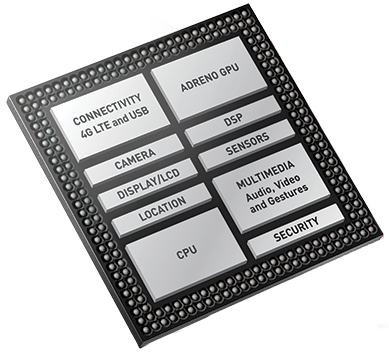
\includegraphics[width=0.65\textwidth]{Figs/qualcomm_snapdragon410_block}\\
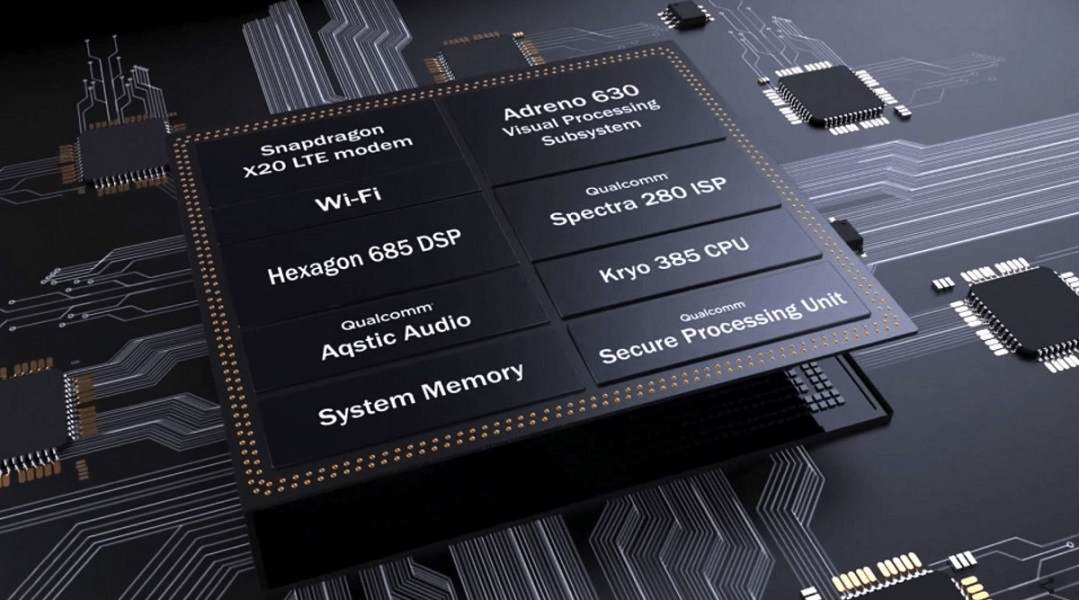
\includegraphics[width=0.85\textwidth]{Figs/Snapdragon-855-1}
     \end{center}
\end{column}
\end{columns}
\end{frame}



\begin{frame}{GPU}
\begin{columns}
\begin{column}{0.70\textwidth}  
\begin{itemize}
\item La mayoría de los teléfonos inteligentes tienen integrado un GPU
\item Un GPU es una unidad especializada de procesamiento para operaciones de punto flotante en paralelo.
\item El Samsung S10 Qualcomm Snapdragon 855 SoC (tiene un CPU de 8 núcleos y un GPU dedidado para gráficos (Adreno 640).
\end{itemize}
\end{column}
\begin{column}{0.30\textwidth}  
    \begin{center}
     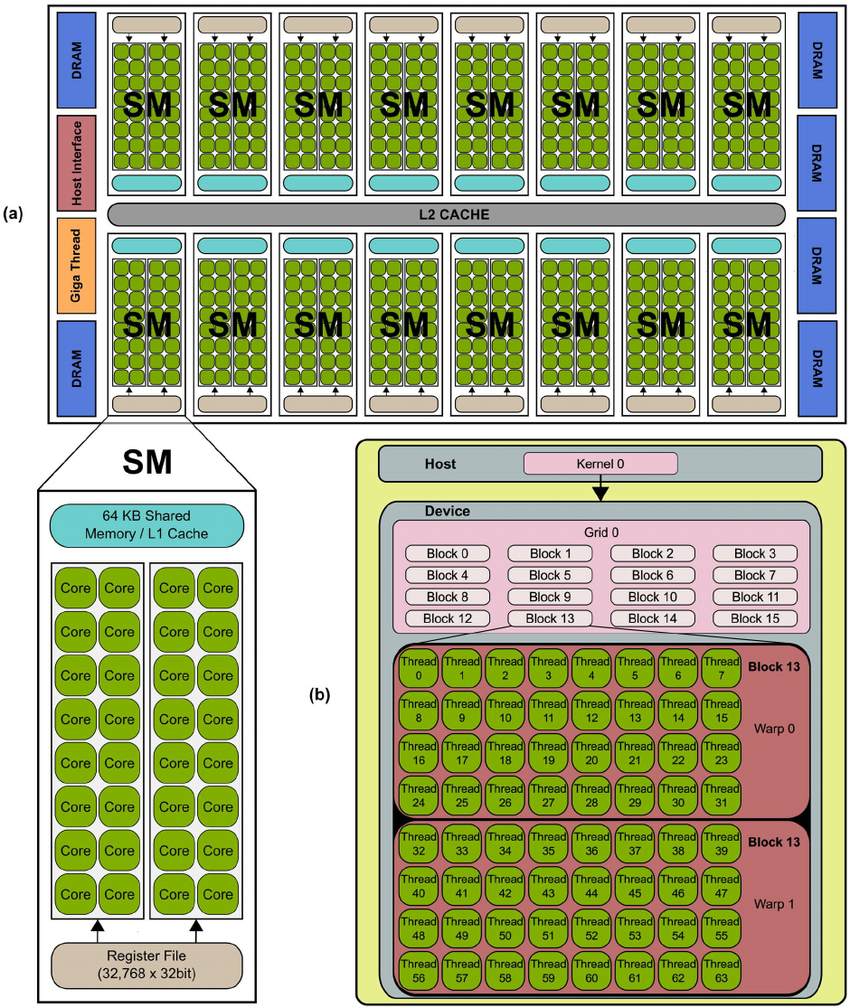
\includegraphics[width=\textwidth]{Figs/Typical-NVIDIA-GPU-architecture}
     \end{center}
\end{column}
\end{columns}
\end{frame}

%\begin{frame}{OpenGL}
%OpenGL signfiica Open Graphics Library, un estándar para la progamación de gráfica.
%El OpenGL Shading Language es un lengauje de alto nivel (cuya sintaxis es parecida a C) diseñado para procesamiento en paralelo en un GPU. 
%\end{frame}


\begin{frame}{CPU-GPU}
\begin{columns}
\begin{column}{0.50\textwidth}  
\begin{itemize}
\item La mayoría de los teléfonos inteligentes tienen integrado un GPU
\item Un GPU es una unidad especializada de procesamiento para operaciones de punto flotante en paralelo.
\item El Samsung S10 Qualcomm Snapdragon 855 SoC (tiene un CPU de 8 núcleos y un GPU dedidado para gráficos (Adreno 640).
\end{itemize}
\end{column}
\begin{column}{0.50\textwidth}  
    \begin{center}
     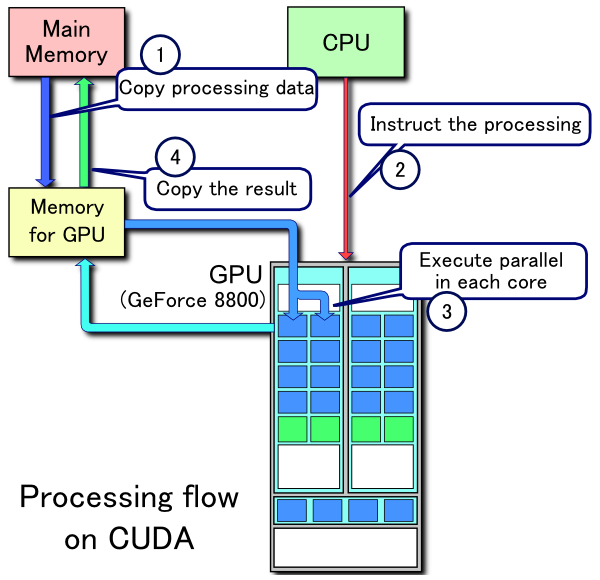
\includegraphics[width=\textwidth]{Figs/CUDA_processing_flow}
     \end{center}
\end{column}
\end{columns}
\end{frame}
